%!TEX program = xelatex
\documentclass[10pt,svgnames,handout]{beamer}
\PassOptionsToClass{svgnames}{xcolor}

\usetheme[progressbar=frametitle]{metropolis}

\metroset{block=fill}

\usepackage{adjustbox}

\usepackage{fontspec}
\setmainfont{Linux Biolinum O}
\setsansfont{Linux Biolinum O}
\setmonofont{Liberation Mono}[Scale=MatchLowercase]

\usepackage{listings}
\lstset{%
  basicstyle=\ttfamily\color{mLightBrown},
  upquote=true,
  keywordstyle=\itshape\color{FireBrick},
  alsoletter={<,>},
  morekeywords={<user>,<project>,<file>,<SHA>}
}

\hypersetup{
  colorlinks=true,
  linkcolor=,
  urlcolor=Teal
}

\usepackage{gitdags}

\graphicspath{{./figures/}}

\usepackage{appendixnumberbeamer}

\usepackage{booktabs}
\usepackage{multirow}

% \usepackage{xspace}
% \newcommand{\themename}{\textbf{\textsc{metropolis}}\xspace}

\title{Git better}
\subtitle{Collaborative project management using \emph{Git} and \emph{GitHub}}
\date{\today}

\author{Matteo Sostero}
\institute{
Workshop @ Modellers Group\\
Sant'Anna School of Advanced Studies}
\date{February 9, 2018} %\\ These slides: \url{http://matteosostero.com/files/slides_git.pdf}}
% \titlegraphic{\hfill\includegraphics[height=1.5cm]{logo.pdf}}

\begin{document}

\maketitle

\begin{frame}
\frametitle{Let's Git it done!}
    
These slides are a brief primer to Git, and how it can help your workflow.

%\bigskip

% \centerline{Find these slides at: \url{https://bit.ly/SA_git}}

\bigskip
\pause

References:
\begin{itemize}
  \item \href{https://www.atlassian.com/git/tutorials}{Atlassian tutorial}
  \item \href{https://guides.github.com/}{GitHub guides}
  \item \href{http://ndpsoftware.com/git-cheatsheet.html}{Git cheatsheet}
  \item \href{https://git-scm.com/book/en/v2}{Git book}
\end{itemize}
\medskip

Troubleshooting:
\begin{itemize}
  \item \href{https://github.com/blog/2019-how-to-undo-almost-anything-with-git}{How to undo (almost) anything with Git}
  \item \href{https://github.com/k88hudson/git-flight-rules/blob/master/README.md}{Git flight rules}
\end{itemize}
\end{frame}

\begin{frame}{Overview}
\setbeamertemplate{section in toc}[sections numbered]
\tableofcontents[hideallsubsections]
\vfill
\end{frame}


\section{Version control with Git}

\begin{frame}
\frametitle{Git}

\includegraphics[height=1cm]{Git-logo}

Git is a distributed version control system for tracking changes in files and coordinating work on those files among multiple people.
\smallskip
\pause

\textbf{Version control} (Git, Mercurial, CVS, Subversion, Bitkeeper):
\begin{itemize}
   \item keep track of changes to text files line-by-line over time;
   \item easily track what changed between any two versions (text);
   \item revert any change if needed;
   \item back up and distribute copies of files;
   \item collaborate on projects.
 \end{itemize} 
\pause
\textbf{Distributed}:
\begin{itemize}
  \item developers keep local copy of entire code and history;
  \item can make changes offline and asynchronously;
  \item changes (easily) reconciled later.
\end{itemize}
\end{frame}


\begin{frame}
\frametitle{Git pros}

Advantages of Git:
\begin{itemize}
  \item widely used, supported, documented;
  \item online platforms: \href{https://github.com/}{GitHub}, \href{https://bitbucket.org/}{Bitbucket}, \href{https://about.gitlab.com/}{GitLab};
  \item dektop interfaces: shell, \href{https://desktop.github.com/}{GitHub Desktop}, \href{https://www.sourcetreeapp.com/}{SourceTree}, \href{https://www.gitkraken.com/}{GitKraken};
  \item integration in editors and IDEs: Emacs, Sublime Text, RStudio, XCode, Visual Studio, \ldots;
  \item distributed (asynchronous, offline) development;
  \item easy branching: eg, experimental branches for trying changes);
  \item easily make complex merges.
\end{itemize}
\end{frame}


\begin{frame}
\frametitle{Let's Git on the same page}
\label{git_cons}

Challenges:
\begin{itemize}
  \item steep learning curve;
  \item \hyperlink{xkcd_git}{complex conceptual model};
  \item cryptic man pages (but good documentation!).
  \item trivial handling of binary files, images, Office documents;
\end{itemize}

\medskip
\pause 

Requires some workflow changes (\hyperlink{style}{see details}):
\begin{itemize}
  \item keep project under single directory (\emph{outside} Dropbox, Google Drive, piCloud, \ldots!)
  \item consistency in personal and team coding style (eg, indentation, spacing, line-breaking);
  \item save and commit changes manually and frequently;
  \item requires to document code and explain changes.
\end{itemize}
\end{frame}


\section{Essential concepts}
\begin{frame}
\frametitle{Git concepts: What}
    
\begin{itemize}[<+->]
\item \textbf{repository} (\textbf{repo}): a collection of files and their history:
\begin{itemize}
   \item where the code is kept: under a single root directory;
   \item can be \textbf{local} (your machine), or distributed across your team or on a \textbf{remote} server (eg, GitHub).
 \end{itemize}

\item \textbf{commit}: a snapshot of your files at a given time:
\begin{itemize}
  \item how Git keeps track of changes in code over time and across team;
  \item manually \lstinline{add} one or more files to include to commit them and describe what changed in a message;
  \item a permanent record of what changed (\lstinline{diff}), when, by whom, with respect to what (\textbf{parent commit});
  \item a repository is “just a directed acyclic graph of commits”.
\end{itemize}
\end{itemize}
\end{frame}

\begin{frame}
\frametitle{Git concepts: Where}

Git has a sophisticated model of \emph{where} things happen, based on how frequently you change things:

\begin{itemize}
\item \textbf{Working directory} (\textbf{working tree, workspace}): the files and sub-directories you can see and work on.\\
\emph{These are visible files stored on your disk.}
\smallskip

\item \textbf{Staging area} (\textbf{index}): where you list files that will go into your next commit.\\
\emph{This is a file in the hidden \texttt{.git/} subdirectory on your disk.}\smallskip

\item \textbf{(local) Repository}: where the commits are stored; ie, it contains the full history of previous versions of the files in the repository, and relevant metadata.\\
\emph{Contained in the hidden \texttt{.git/} subdirectory on your disk.}
\smallskip

\item \textbf{(remote) Repository}: a version of the repository hosted elsewhere.\\
\emph{On another computer, or online service like GitHub or Bitbucket.}
\end{itemize}
\end{frame}


\begin{frame}
\frametitle{Life cycle of files in a repository: from changes to staging area}
\begin{centering}
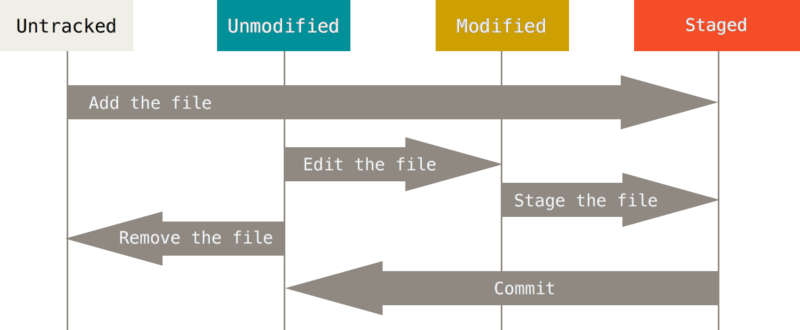
\includegraphics[width=\linewidth]{figures/lifecycle.png}
\end{centering}
\end{frame}


\begin{frame}
\frametitle{Key commands: repository actions}

\begin{itemize}[<+->]
\item \lstinline{git status} (or interface) tells you the state of your repository:
\begin{itemize}
  \item which files are \textbf{untracked} and not indexed.
  \item which files are \textbf{modified} with respect to the index/staging area;
  \item which files are \textbf{staged} (\textbf{indexed}) and ready to be commited;
\end{itemize}
\item \lstinline|git add| new or modified files to the index.
\item \lstinline|git commit| commits changes in the index.
\bigskip
\item \lstinline{git diff} shows what has changed, wrt index or last commit.
\item \lstinline{git log} shows the history of commits up to this point.
\bigskip
\item \lstinline|git push|: send your local changes to the remote server;
\item \lstinline|git pull| (\lstinline{git fetch}; \lstinline{git merge}): get latest changes from remote.
\bigskip
\item \lstinline|git clone|: copy a remote repository on your machine;
\item \lstinline|git init|: start a new repository in empty directory;
\end{itemize}
\end{frame}


\begin{frame}
\frametitle{Example workflow 1}

\begin{block}{Solitary development, offline, from scratch}
    
\begin{enumerate}
  \item create a new empty directory on your computer
  \item \lstinline|git init|: create a Git repository in the directory
  \item create, edit, and save some \texttt{file.txt} in the directory
  \item \lstinline|git status| shows the file is untracked
  \item \lstinline|git add file.txt| to stage the file
  \item \lstinline|git commit -m "First commit! added file.txt!"|
  \item \lstinline|git status| reports no changes
  \item edit the file again, repeat from step (4).
\end{enumerate}
\end{block}
\end{frame}

%TODO: animate.
\begin{frame}
\frametitle{Working with repositories: from changes to commits}
\input{./figures/git_workflow.fig}\\
\begin{small}
Adapted from \href{https://tex.stackexchange.com/a/70332/14260}{Stackoverflow}. See also \href{http://ndpsoftware.com/git-cheatsheet.html}{ndpsoftware.com/git-cheatsheet.html}
\end{small}

\end{frame}



\section{History and branching}

\begin{frame}
\frametitle{History of the repo with \lstinline{git log}}

\lstinline{git log} (or the interface) shows the history of commits of the repo: \pause

\begin{block}{Log of a solitary development workflow}
\input{./figures/history_linear.fig}
\end{block}
\smallskip
\pause
Note:
\begin{itemize}
  \item commits are uniquely identified by a SHA-1 hash (eg, \texttt{a12b34\ldots});
  \item commit messages can have two parts:
  \begin{itemize}
    \item short description ($\sim<50$~characters, above)
    \item details after two line break (not shown);
  \end{itemize}
  \item \lstinline{HEAD} means “where your next commit would go” (pointer to branch);
  \item \lstinline{Master} is the name of the main \textbf{branch}
\end{itemize}
\end{frame}


\begin{frame}
\frametitle{Branches}

\textbf{Branches} are sequences of commits, which can trace an alternative history and versions of the code in yout repo.\\
\begin{itemize}
  \item there is always a \lstinline{Master} branch, containing the \emph{main}, \emph{baseline} version of the code.
  \item Git makes creating and merging branches quick and easy: it's a great help to the worflow.
  \item other branches can be created from any commit to \emph{experiment}, \emph{implement new features}, \emph{keep diverging versions}.
\end{itemize}
\pause

\begin{block}{Example history with branches}
\input{./figures/history_branch.fig}
\end{block}

\end{frame}


\begin{frame}
\frametitle{Moving across branches with \lstinline{git checkout}}

\lstinline{git checkout} moves \lstinline{HEAD} on the tree (different branch or earlier commit on the same branch): it shows the files at  different commit.\\
\medskip
\pause

\begin{block}{Example switching branches}
\begin{tikzpicture}[scale=0.9]
% Commit DAG
\gitDAG[grow right sep = 2em]{
  A -- B -- { 
    C,
    D -- E,
  }
};

% Master branch
\gitbranch{master}{right=of C}{C}

% Feature branch
\gitbranch{feature}{right=of E}{E}

% HEAD reference
\gitHEAD{right=of feature}{feature}
\end{tikzpicture}

\pause
\lstinline{git checkout master}
\pause

\begin{tikzpicture}[scale =0.9]
% Commit DAG
\gitDAG[grow right sep = 2em]{
  A -- B -- { 
    C,
    D -- E,
  }
};
% Master branch
\gitbranch{master}{right=of C}{C}
% Feature branch
\gitbranch{feature}{right=of E}{E}
% HEAD reference
\gitHEAD{right=of master}{master}
\end{tikzpicture}

\end{block}
\end{frame}



\begin{frame}
\frametitle{Merging branches with \lstinline{git merge}}

From the \lstinline{Master} branch, \lstinline{git merge feature master} creates a new commit combining the two branches.

\begin{block}{Merging branches}
\lstinline{git checkout master}

\begin{tikzpicture}[scale =0.9]
% Commit DAG
\gitDAG[grow right sep = 2em]{
  A -- B -- { 
    C,
    D -- E,
  }
};

% Master branch
\gitbranch{master}{right=of C}{C}
% Feature branch
\gitbranch{feature}{right=of E}{E}
% HEAD reference
\gitHEAD{right=of master}{master}
\end{tikzpicture}

\medskip
\pause
\lstinline{git merge feature master}

\begin{tikzpicture}[scale=0.9]
% Commit DAG
\gitDAG[grow right sep = 2em]{
  A -- B -- { 
    C -- F[xshift=10mm],
    D -- E -- F[xshift=10mm],
  }
};
% Master branch
\gitbranch{master}{right=of F}{F}
% Feature branch
\gitbranch{feature}{right=of E}{E}
% HEAD reference
\gitHEAD{right=of master}{master}
\end{tikzpicture}


\end{block}
\end{frame}

% \section{Undoing anything}

\section{Collaborative development}

\begin{frame}
\frametitle{Collaborating on remote git repositories (GitHub, Bitbucket,\ldots)}
Online hosting services like GitHub and Bitbucket provide:
\begin{itemize}[<+->]
  \item \textbf{remote repository} to back up code;
  \item \textbf{issue tracking} interface: reporting bugs, suggesting improvements;
  \item \textbf{project and team management}: decide who can do what;
  \item managing contributions (\textbf{pull requests}) from team members and third parties;
  \item place to \textbf{host documentation} and \textbf{share know-how} on the code;
  \item venue to \textbf{make code public} and \textbf{invite collaboration} from anyone.
\end{itemize}
\pause

\begin{center}
\includegraphics[width=0.5\linewidth]{GitHub_poster.jpg}
\end{center}
\end{frame}

\begin{frame}
\frametitle{Collaboration workflow on remote git repositories}
The typical workflow within our GitHub \emph{organization} or Bitbucket \emph{team} would be:
\begin{enumerate}[<+->]
  \item create a (private/public) repository within the organization.
  \begin{itemize}
    \item invite collaborators among modelers;
    \item nominate administrators, maintainers, access rights, etc.
  \end{itemize}
  \item upload (or migrate) existing code on the repository;
  \item other modelers clone repository on their machine, replicate and experiment;
  \item document existing code; add a \texttt{README.md} explaining what the model does, reference to papers, how to collaborate;
  \item document issues, suggest improvements;
  \item create branches for developing new versions (features, bugfix,\ldots)
  \item merge branches in \texttt{Master} to integrate in the development version.
  \item tag specific commits to refer to milestones of the project.
\end{enumerate}

\end{frame}



\section{Coding with style}

\begin{frame}
\label{style}
\frametitle{Git with style}

Some matters of style and workflow to collaborate with ease.

\begin{itemize}[<+->]
\item repository as self-contained, dedicated directory of (mostly) code:
\begin{itemize}
  \item include \textbf{all} relevant files in the repo (libraries, dependencies, \ldots);
  \item in your code, refer to dependencies using relative paths: \lstinline{./library/}, \textbf{not} \lstinline{/home/user/project_name/library};
  \item exclude unnecessary files (eg, compilation artifacts, large data, useless binary files) using \texttt{.gitignore} (see \href{https://github.com/GitHub/gitignore}{github.com/GitHub/gitignore}).
  \item keep it \textbf{outside} shared folders of Dropbox, Google Drive, piCloud!
\end{itemize}
\item be \textbf{consistent} in personal and team coding style: indentation/tabs, spacing, character encoding (UTF-8), line-breaking.
\item conform to a language \textbf{style guide} (eg, \href{https://google.GitHub.io/styleguide/}{google.GitHub.io/styleguide/});
\item \textbf{commit early and often};
\item \textbf{never commit broken code}! use \href{https://git-scm.com/book/it/v2/Git-Tools-Stashing-and-Cleaning}{\lstinline{git stash}} to save it instead.
\item commit related files together;
\item write meaningful commit messages.
\item tag release (baseline, published) versions of your code with \lstinline{git tag}.
\end{itemize}

\end{frame}


% \section{Pricing plans}

% \begin{frame}
% \frametitle{Organization pricing plans}

% Git is free software, but extensive access to the cloud platform (GitHub, Bitbucket,\ldots) is paying for non-open-source projects.

% \small

% \begin{tabular}{llp{6cm}}
% \multicolumn{3}{l}{\textbf{GitHub}}\\
% \toprule
% cloud       & \emph{Education}  & free for education, (max 10 repos)                       \\
% cloud       & \emph{Team}       & from \$25/month (5 users) + \$9/user/month               \\
% cloud       & \emph{Business}   & \$21 per user/month                                      \\
% \midrule
% self-hosted & \emph{Enterprise} & \$21 per user/month (by $\times$10 users, annual) \\
% \bottomrule
% \end{tabular}

% \medskip

% \begin{tabular}{lll}
% \multicolumn{3}{l}{\textbf{Bitbucket}}\\
% \toprule
% cloud       & \emph{Standard} & \$10/month + \$2 per user/month \\
% cloud       & \emph{Premium}  & \$25/month + \$5 user/month     \\
% \midrule
% self-hosted &                 & \$1800/year (25 users)          \\
% self-hosted &                 & \$3300/year (50 users)          \\
% \bottomrule
% \end{tabular}
% \end{frame}


\section{Managing a single-user project locally and remotely on GitHub}

\begin{frame}
\frametitle{Existing project: local and remote repo}
Use case: an existing local project in \lstinline{/<project>/}, as yet untracked by git.

\begin{block}{Workflow}
\begin{itemize}
  \item initialise a git repo:
  \begin{itemize}
    \item \lstinline{cd <project>/}
    \item \lstinline{git init}
  \end{itemize}
  \item create \lstinline{.gitignore} file, exclude irrelevant files.
  \item stage all (relevant) files: \lstinline{git add .}
  \item \lstinline{git status} (is your friend)
  \item commit changes \lstinline{git commit -m "First commit (better late than never)"}
\end{itemize}
\end{block}
\end{frame}

\begin{frame}
\frametitle{Existing project: local and remote repo (continued)}

\begin{block}{Workflow (continued)}
\begin{itemize}
  \item create an \textbf{empty} remote repo called \lstinline{<project>} in GitHub:
  \begin{itemize}
    \item uncheck “Initialize this repository with a README”
    \item no gitignore
    \item no licence
  \end{itemize}
  (You can always add those later; should not commit at this time)

  \item GitHub project now at \lstinline{https://github.com/<user>/<project>}; name need not be globally unique (GUID: \lstinline{<user>/<project>}),\\ but make it \textbf{memorable}, \textbf{evocative} and \textbf{google-able}.

  \item locally, add remote repo address called “origin”: \\ {\small \lstinline{git remote add origin https://github.com/<user>/<project>.git}}

  \item push changes for the first time (creates remote \lstinline{master} branch) :
  \lstinline{git push -u origin master}
\end{itemize}
\end{block}
\end{frame}



\section{Collaborating on team projects on GitHub}
\begin{frame}
\frametitle{Collaborating on a GitHub project}
Use case: working with your team on \lstinline{github.com/<user>/<project>}.

\begin{block}{Workflow}
\begin{enumerate}[<+->]
  \item add collaborators from \lstinline{github.com/<user>/<project>/settings/collaboration};\\
  they receive and accept invitations to work on the repo.
  \item collaborators can access a private repository, clone repository locally and make changes;
  \item collaborators can now push commits to repo, including \lstinline{master}!\\Protect it from foolishness in \lstinline{/settings/branches/} by requiring \textbf{branching} and \textbf{pull requests} in order to commit on \lstinline{master}:
  \begin{itemize}
    \item \textbf{collaborators}—branch $\rightarrow$ commit(s) $\rightarrow$ pull request;
    \item \textbf{repo admin(s)}—evaluate pull requests.
  \end{itemize}
\end{enumerate}
\end{block}
\end{frame}


\section{Undo (almost) anything with Git}
\begin{frame}
\frametitle{How to undo (almost) anything with Git}

Git allows to undo most actions easily, depending on state of the repo.
\pause
\begin{block}{Golden rules}
\begin{itemize}
  \item \textit{Don't Panic!} Your code is still there (somewhere).
  \item working \hyperlink{style}{\textcolor{Teal}{methodically}} will prevent (most) mishaps.
  \item remote commits are there to stay—but you can revert their effects.
\end{itemize} 
\end{block}
\pause
See also:
\begin{itemize}
  \item GitHub's \href{https://github.com/blog/2019-how-to-undo-almost-anything-with-git}{\textit{How to undo (almost) anything with Git}};
  \item \href{https://stackoverflow.com/questions/tagged/git}{Stack Overflow} (pro tip: there is usually $>1$ way to do it).
\end{itemize}
\end{frame}

\begin{frame}
\frametitle{How to undo (almost) anything with Git: examples}
Solutions to \textbf{local} (ie, not-yet-pushed) problems:
\begin{itemize}[<+->]
  \item undo changes in \lstinline{<file>} made since last commit: return files to last commit with \lstinline{git checkout -- <file>};
  \item undo changes just committed (eg, typo in message or error in code): fix files, add them and commit again with \lstinline{--amend} option;
  \item stop tracking \lstinline{<file>}: \lstinline{git rm --cached <file>}; add it to \lstinline{.gitignore}; commit;
  \item undo changes in several recent commits: return to last good commit with \lstinline{git log}, look for \lstinline{<SHA>} of commit, then \lstinline{git reset <SHA>}
\end{itemize}
\medskip
\pause
Solutions to \textbf{public} (ie, pushed to remote) problems:
\begin{itemize}
  \item undo a public commit \lstinline{<SHA>}: \lstinline{git revert <SHA>} will create a new commit, that undoes (inverts) the changes in introduced by \lstinline{<SHA>}; this new commit is added to existing (public) history.
\end{itemize}

\end{frame}


\section{Contributing to third-party open-source projects on GitHub}
\begin{frame}
\frametitle{Contributing to third-party repositories on GitHub}
GitHub hosts many great projects, mostly managed by volunteers. \\
\medskip
\pause
Here's how you can help:
\begin{itemize}[<+->]
\item \textbf{report issues (bugs)}: 
\begin{itemize}
  \item \textbf{first, due diligence}: read documentation, search existing issues, repo Wiki, StackOverflow answers. Is your problem really new or general?
  \item describe all the steps needed to reproduce; embed example code in Markdown (eg, \href{https://stackoverflow.com/questions/5963269/how-to-make-a-great-r-reproducible-example}{R Minimal Reproducible Example});
  \item give feedback on proposed solutions.
\end{itemize}
\item \textbf{fix issues}: if you can solve an existing issue, fork the repo, work on it, and submit a pull request.
\item \textbf{documentation}: writing good documentation takes time, and developers may be happy to delegate. Ask how you can help.
\item \textbf{say thanks}: volunteer development is a thankless task; reach out to thank to the developers on social media.
\end{itemize}
\end{frame}


\section{Further topics}
\begin{frame}
\frametitle{Sharing snippets of code easily with GitHub Gists}
GitHub Gists (\href{https://gist.github.com/}{gist.github.com}) are pages to store and share snippets of code. They are light-weight repositories, with an emphasis on showcasing the code itself, and making it easy to copy.\\
\pause
\begin{itemize}
  \item great for sharing self-contained scripts or config files;
  \item automatically highlight code and can embed it in third-party websites;
  \item can be edited online by the author (automatic versioning);
  \item either public (listed on your profile page, searchable) or private (access with link only);
  \item can gather comments from everyone.
\end{itemize}
\end{frame}
\begin{frame}


\frametitle{References to advanced topics}
Some useful topics covered in GitHub Guides (\href{https://guides.github.com/}{guides.github.com}):
\begin{itemize}
  \item \href{https://guides.github.com/features/mastering-markdown/}{Mastering Markdown}: all about GitHub-flavoured Markdown, the easiest mark-up language around—used extensively in GitHub READMEs, issues, comments, and around the web;
  \item \href{https://guides.github.com/features/wikis/}{Documenting your projects on GitHub}: writing great documentation (README, Wiki, pages) for your repo (in Markdown);
  \item \href{https://guides.github.com/activities/citable-code/}{
Making Your Code Citable}: assign a \textsc{doi} (Digital Object Identifier) to cite your code in academic publication, using GitHub and \href{https://zenodo.org/}{Zenodo};
  \item \href{https://guides.github.com/features/pages/}{GitHub Pages}: easily build a website from a GitHub repo—for your project or for yourself!
\end{itemize}
\end{frame}

% \begin{frame}
% \frametitle{Configuring Sublime Text for \LaTeX{} and Git}
% \end{frame}


\begin{frame}<handout:0>[standout]
Thank you!
\end{frame}


\appendix

\begin{frame}<handout:0>
\label{xkcd_git}
\frametitle{XKCD on git \hfill\hyperlink{git_cons}{\beamergotobutton{back}}}

\begin{columns}[T,onlytextwidth]
\column{0.45\textwidth}

\includegraphics[width=\textwidth]{figures/xkcd-git.png}

\column{0.45\textwidth}
\vfill
\emph{If that doesn't fix it, git.txt contains the phone number of a friend of mine who understands git.
Just wait through a few minutes of “It's really pretty simple, just think of branches as\ldots” and eventually you'll learn the commands that will fix everything.
}
\end{columns}
\end{frame}
\end{document}
